% !TEX root = ./ICDE14_conf_full_296.tex
\section{\hl{Selection of Geospatial Data}}
\label{sec:background}

\hl{In the }\emph{\hl{selection problem,}}\hl{ we wish to select the subset of a geospatial dataset to be visualized on a map at a given scale}. Below we define the basic components of the problem, and informally define the associated optimization problem.

\subsection{Geospatial records and weights}
\label{sec:records}

The dataset is assumed to consist of a set of \emph{geospatial records} drawn from a database table. The schema of a geospatial record consists of a \emph{geometry} field (e.g. a point, line or polygon), a \emph{unique ID} field and any number of additional textual and numeric fields, such as ``city name'' and ``population''.

Each record is assigned a \emph{user defined weight} using CVL (see Section~\ref{sec:cvl:language}). \hl{The weight models the importance of a record, with high weight corresponding to great importance}. Any subset of records --- or all records for that matter --- may have the same weight. Therefore, the weights induce a partial order of the records.

\subsection{Zoom levels and map constraints}
\label{sec:constraints}
\hl{For zoomable maps, different subsets of the data should be selected for display at different scales or }\emph{zoom levels}. Let the zoom-levels run from 1 (lowest scale) to $\mathcal{Z}$ (largest scale). On a given zoom level, the map is rendered at a certain pixel resolution. Thus, for a given zoom level, we know the distance in pixels between geospatial locations. This gives rise to two particularly important map constraints~\cite{harrie2007modelling} \hl{when selecting data for a given zoom level}.

Firstly, the \emph{principle of constant information density} implies that the number of records that can be displayed \hl{within an area of a certain pixel size should be bounded}~\cite{topfer1966principles}. Assume that we divide the complete map into cells (or tiles) of, say, 256 x 256 pixels. The \emph{visibility} constraint states that each cell can contain at most $K$ \hl{selected} records, where $K$ is a user-defined parameter~\cite{sarma2012fusiontables}.

Secondly, records cannot be too close to each other in the map --- otherwise the user will not be able to \hl{clearly distinguish between them}. The \emph{proximity} constraint states that every pair of visible records must be separated by at least $d$ pixels, where $d$ is a user defined parameter.

In addition to these constraints that must hold separately for each zoom level, there are constraints that must hold across zoom levels. A particularly important constraint is the \emph{zoom-consistency} constraint, which states that when a record is filtered out at a given scale, it should also be filtered out at all \emph{lower} scales~\cite{sarma2012fusiontables}. When a user zooms out on a map, records can only disappear --- not reappear.

Apart from the zoom-consistency constraint, \hl{CVL supports constraints based on }\emph{simple measures}\hl{ that are }\emph{satisfiable by selection} (see Section~\ref{sec:cvl:language}).\hl{ A simple measure is a function that maps a set of records to a scalar value. A constraint is violated if the measure exceeds a threshold. A constraint is satisfiable by selection if we can }\emph{always}\hl{ satisfy it by simply deleting an appropriate subset of the records. Both the visibility and proximity constraints respect these restrictions. However, we cannot model constraints that have complex measures or cannot be satisfied by using selection alone, such as }\emph{topology}\hl{ and }\emph{spatial distribution}\hl{ constraints. We leave these classes of constraints to future work.}

\subsection{\hl{Conflicts}}
\label{sec:conflicts}

\hl{Constraints such as visibility or proximity can be modeled using the notion of }\emph{conflicts}. \hl{A conflict is a set of records that cannot all be selected without violating the constraint}.

\hl{For the visibility constraint, there is a conflict generated for every cell that contains more than $K$ records. For the proximity constraint, there is a conflict generated for each pair of records that is less than $d$ pixels apart (see Figure}~\ref{fig:proximity:conflict}\hl{)}. A record can be in several \hl{conflicts}, which is the case for point $p$ in the example shown in the figure. \hl{A solution to the selection problem is }\emph{feasible}\hl{ if there are no conflicts}.

\begin{figure}[htbp]
\begin{center}
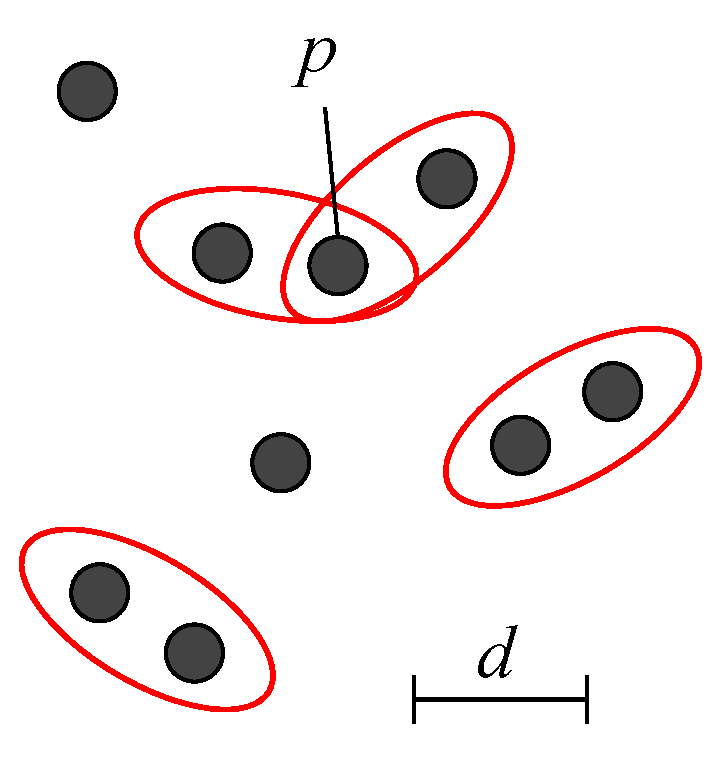
\includegraphics[scale=.3]{figs/cvl_proximity_conflicts.pdf}
\caption{Conflicts generated by the proximity constraint for distance $d$. Notice that point $p$ is a member of more than one \hl{conflict}.}
\label{fig:proximity:conflict}
\end{center}
\vspace*{-4ex}
\end{figure}

Consider a \hl{conflict involving} $k_1$ records, where at most $k_2$ of these records can be selected (where $k_1 > k_2$). Then it is equivalent to state that at least $\lambda = k_1 - k_2$ of these records must be \emph{deleted}. In the mathematical formulation of the problem in Section~\ref{sec:optimizationmodel}, we will use this alternative way to formulate \hl{conflicts}.

\subsection{\hl{Selection as an optimization problem}}
\label{sec:filtering}
\hl{The notion of conflicts is used to define the feasibility of solutions to the selection problem. This should be accompanied by a way to discriminate between solutions. Assigning an importance measure to each record, namely the record weights, intuitively allows us to measure the ``loss of importance'' due to records that are deleted.} 

\hl{In the optimization version of the problem, we seek the feasible solution that minimizes the aggregate weight of records that are deleted. In Section}~\ref{sec:optimizationmodel}\hl{, we present a mathematical formulation of the selection optimization problem}.

\hl{For a zoomable map with }$\mathcal{Z}$\hl{ zoom levels, we are interested in finding $\mathcal{Z}$ solutions to the selection problem, one for each zoom level }$i \in \{ 1, \ldots, \mathcal{Z} \}$. \hl{We call this problem the }\emph{multi-scale selection problem}. \hl{To control the way in which we compute these solutions, we use an algorithmic framework known as the }\emph{ladder} approach~\cite{foerster2010challenges}. \hl{This is a recursive approach, where the output of selection at large scale is used as input to selection at a smaller scale. This means that the zoom-consistency constraint }(Section~\ref{sec:constraints})\hl{ is automatically satisfied}.

\hl{The ladder approach is not appropriate for all use cases. For example, when regional labels are modeled as geospatial records, e.g., the label ``Europe'', we may wish to show a record only on intermediate zoom levels, violating zoom consistency. Handling these use cases would require an alternative formulation, e.g., following the }\emph{star} \hl{approach}~\cite{foerster2010challenges}. \hl{This is an interesting avenue for future work}.  

% should be visible mostly on the intermediate zoom levels, the }\emph{star} approach~\cite{foerster2010challenges}\hl{ would be better. This is a limitation of the work presented in this paper.}



